%!TEX root = Thesis.tex
\chapter{Implementation and Evaluation}
The chapter presents a prototype of the reference scenario considered in the section
2.3. The prototype implements the major aspects proposed in the concept (chapter
4).
%%%%%%%%%%%%%%%%%%%%%%%%%%%%%%%%%%%
\section{Overview of Framework}
\section{Web-based Framework Analysis}
 \begin{itemize}
\item \textbf{Bootstrap}
\newline
Bootstrap is the most popular and widely used framework, nowadays. It’s a beautiful, intuitive and powerful web design kit for creating cross browser, consistent and good looking interfaces. It offers many of the popular UI components with a plain-yet-elegant style, a grid system and JavaScript plugins for common scenarios.

It is built with LESS and consists of four main parts:
Scaffolding – global styles, responsive 12-column grids and layouts. Bear in mind that Bootstrap doesn’t include responsive features by default. If design needs to be responsive this functionality have to be done manually.
Base CSS – this includes fundamental HTML elements like tables, forms, buttons, and images, styled and enhanced with extensible classes.
Components – collection of reusable components like dropdowns, button groups, navigation controls (tabs, pills, lists, breadcrumbs, pagination), thumbnails, progress bars, media objects, and more.
JavaScript – jQuery plugins which bring the above components to life, plus transitions, modals, tool tips, popovers, scrollspy (for automatically updating nav targets based on scroll position), carousel, typeahead (a fast and fully-featured autocomplete library), affix navigation, and more.
\item \textbf{Foundation}
\newline
Foundation is a powerful, feature-rich, responsive front-end framework. With Foundation user can quickly prototype and build websites or apps that work on any kind of device, with tons of included layout constructs, elements and best practices. It’s built with mobile first in mind, utilitizes semantic features, and uses Zepto instead of jQuery in order to brings better user experience and faster performance.

Foundation has a 12-column flexible, nestable grid powerful enough to create rapidly multi-device layouts. In terms of features it provides many. There are styles for typography, buttons, forms, and various navigation controls. Many useful CSS components are provided like panels, pricing tables, progress bars, tables, thumbnails, and flex video that can scale properly your video on any device. And, of course, JavaScript plugins including dropdowns, joyride (a simple and easy website tour), magellan ( a sticky navigation that indicates where is the user on the page), orbit (a responsive image slider with touch support), reveal (for creating modal dialogs or pop-up windows),  sections (a powerful replacement for traditional accordions and tabs), and tooltips.
\item \textbf{GroundworkCSS}
\newline
GroundworkCSS is a new, fresh addition to the front-end frameworks family. It’s a fully responsive HTML5, CSS and JavaScript toolkit built with the power of Sass and Compass which gives the ability to rapidly prototype and build websites and apps that work on virtually any device.

It offers an extremely flexible, nestable, fraction-based, fluid grid system that makes creating any layout possible. GroundworkCSS has some really expressive features like tablets and mobile grids which maintain the grid column structure instead of collapsing the grid columns into individual rows when the viewport is below 768 or 480 pixels wide. Another cool feature is a jQuery ResponsiveText plugin which allows to have dynamically sized text that adapts to the width of the viewport: extremely useful for scalable headlines and building responsive tables.
The framework includes a rich set of UI components like tabs, responsive data tables, buttons, forms, responsive navigation controls, tiles (a beautiful alternative to radio buttons and other boring standard form elements), tooltips, modals, Cycle2(a powerful, responsive content slider), and many more useful elements and helpers. It also offers a nice set of vector social icons and a full suite of pictographic icons included in FontAwesome.
To see the framework in action user can use the resizer at the top center of the browser window. This way user can test the responsiveness of the components against different sizes and viewports while exploring the framework’s features.
GroundworkCSS is very well documented with many examples, and to get user started quickly the framework also provides several responsive templates. The only thing as a weakness is the missing of a way to customize download.

\item \textbf{Gumby}            
\newline
Gumby is simple, flexible, and robust front-end framework built with Sass and Compass.

Its fluid-fixed layout self-optimizes the content for desktop and mobile resolutions. It support multiple types of grids, including nested ones, with different column variations. Gumby has two PSD templates that get user started designing on 12 and 16 column grid systems.
The framework offers feature-rich UI Kit which includes buttons, forms, mobile navigation, tabs, skip links, toggles and switches, drawers, responsive images, retina images, and more. Following the latest design trends the UI elements have Metro style flat design but can use Pretty style with gradient design too, or to mix up both styles. An awesome set of responsive, resolution independent Entypo icons, is completely integrated into the Gumby Framework. Gumby has also a very good customizer with color pickers which helps to build your custom download with ease.
\item \textbf{Kube}
\newline
Lastly, if user need a solid, yet simple base without needless complexity and extras, for your new project, Kube can be the right choice. Kube is a minimal, responsive and adaptive framework with no imposed styling which gives to user the freedom to create. It offers basic styles for grids, forms, typography, tables, buttons, navigation, and other stuff like links or images.

The framework contains one compact CSS file for building responsive layouts with ease and two JS files for implementing tabs and buttons in your designs. If user is looking for maximum flexibility and customization, user can download developer version which includes LESS files, with variables, mixins and modules.
\end{itemize}

\begin{figure}[!ht]
\centering
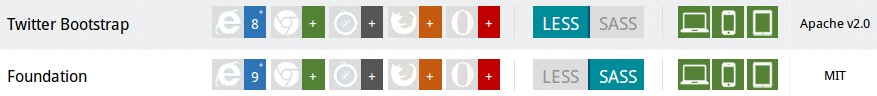
\includegraphics[scale=0.7]{images/Bootstrap&Foundation.png}
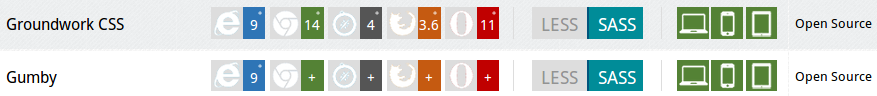
\includegraphics[scale=0.7]{images/Groundwork&Gumby.png} 

\includegraphics[scale=0.7]{images/Kube.png}  
\caption[Framework Comparison]{Framework Comparison\footnote{\url{http://usablica.github.io/front-end-frameworks/compare.html}}}
\label{img:Bootstrap&Foundation.png}
\label{img:Groundwork&Gumby.png}   
\label{img:Kube.png}                          
\end{figure}
\section{Data Flow Model}
\subsection{XMPP BOSH Client}
The Extensible Messaging and Presence Protocol (XMPP) is the IETF’s formalization of the base XML streaming protocols for instant messaging and presence developed within the Jabber community starting in 1999. This page provides a brief chronology of Jabber/XMPP technologies from the perspective of standardization\cite{xmpp}.
\newline
\emph{Decentralization}
\newline
The architecture of the XMPP network is similar to email; anyone can run their own XMPP server and there is no central master server.
\newline
\emph{Open standards}
\newline
The Internet Engineering Task Force has formalized XMPP as an approved instant messaging and presence technology under the name of XMPP (the latest specifications are RFC 6120 and RFC 6121). No royalties are required to implement support of these specifications and their development is not tied to a single vendor.
\newline
\emph{History}
\newline
XMPP technologies have been in use since 1999. Multiple implementations of the XMPP standards exist for clients, servers, components, and code libraries.
\newline
\emph{Security}
\newline
XMPP servers can be isolated from the public XMPP network (e.g., on a company intranet), and strong security (via SASL and TLS) has been built into the core XMPP specifications.
\newline
\emph{Flexibility}
\newline
Custom functionality can be built on top of XMPP; to maintain interoperability, common extensions are managed by the XMPP Standards Foundation. XMPP applications beyond IM include groupchat, network management, content syndication, collaboration tools, file sharing, gaming, remote systems control and monitoring, geolocation, middleware and cloud computing, VoIP and Identity services.
The XMPP network uses a client–server architecture (clients do not talk directly to one another). However, it is decentralized—by design, there is no central authoritative server, as there is with services such as AOL Instant Messenger or Windows Live Messenger. Some confusion often arises on this point as there is a public XMPP server being run at jabber.org, to which a large number of users subscribe. However, anyone may run their own XMPP server on their own domain.
Every user on the network has a unique Jabber ID (usually abbreviated as JID). To avoid requiring a central server to maintain a list of IDs, the JID is structured like an email address with a username and a domain name (or IP address[16]) for the server where that user resides, separated by an at sign (@), such as username@example.com.

\section{Browther Support}
In past years a Flash-based media player in more than sufficient for streaming on the Web and this technology is still necessary to support legacy browsers. But thankfully modern standards have advanced and the inclusion of HTML5 video opens doors for dozens of new opportunities.

In this guide I’d like to offer an introduction to HTML5 video for the Web. It will take some practice to understand the native in-browser player and all its functionality. When you’re working with a flash video player it’s all too common to associate all video formats in .flv. While this does work, most flv files cannot retain quality anywhere near the more advanced file formats/codecs. There are 3 important video types which are supported by HTML5: MP4, WebM, and Ogg/Ogv. The MPEG-4 file type is generally encoded in H.264 which allows for playback in third party Flash players. This means you don’t need to keep a .flv video copy to support a fallback method! WebM and Ogg are two much newer file types related to HTML5 video. Ogg uses Theora encoding which is based on the open-source standard audio file format. These can be saved with a .ogg or .ogv extension.
So which of these file types do you need for your website? Well ideally all 3 would be great as they provide the full support spectrum. Yet this isn’t realistic, and in fact, you can cover all the bases with only two of them. Here is a breakdown of what works for each browser:

Mozilla Firefox – WebM, Ogg
Google Chrome – WebM, Ogg
Opera – WebM, Ogg
Safari – MP4
Internet Explorer 9 – MP4
Internet Explorer 6-8 – No HTML5, Flash Only!
Most flash video players will support MP4 files as long as they’re encoded in H.264. As such, each of these browsers will embed MP4+Flash as a final resort. This means you only need to create two different video formats to support all browsers. MP4 for Safari/IE9 and a choice between WebM or Ogg for the rest.
\section{Database Model}
\section{Use Cases}
  \subsection{Frontend}
  \subsection{3-tier Architecture in Software Projection}
  \subsection{Evaluation}
  \subsection{Use Cases Realization}
\subsection{Summary}